\chapter{Results}

%Results. Describe your results in a logical order: this may not necessarily be the order in which you did the experiments. Briefly summarise the main results at the end of each main experiment or sequence of associated experiments. Do not duplicate results -- put a table or a graph but not both unless the two methods of presentation demonstrate different points of importance. You must refer appropriately to figures or tables in the text and remember to emphasise and perhaps quote significant results. In particular, think about:

%o What were the results of your hypothesis tests, in the order you describe them in the Methods?
{\texorpdfstring
%TTo verify the fitting procedure for each of the three models (Classic, Depth, Perimeter) I created three different model simulations. I ran the simulation data through three NLLS fitting scripts to retrieve the known parameters ($\theta$, as calculated from \textit{nu} and metacommunity size \textit{J*K}, \textit{m\textsubscript{0}} and \textit{K}). Here I have plotted the know parameters against those estimated by the model fitting procedure. Once the model fitting procedures are validated, I use them to fit the three models to my datasets, as well as calculating critical area (\textit{A\textsubscript{crit}}) between niche-structured regime and colonisation-extinction regime. Using critical area estimates I test the hypothesis that regime change will occur at lower areas for more motile species and less isolated habitats. 

\section\section{Simulation}

\begin{figure}[htbp]
\centering
\subfloat[The Classic Model]{\label{fig:a}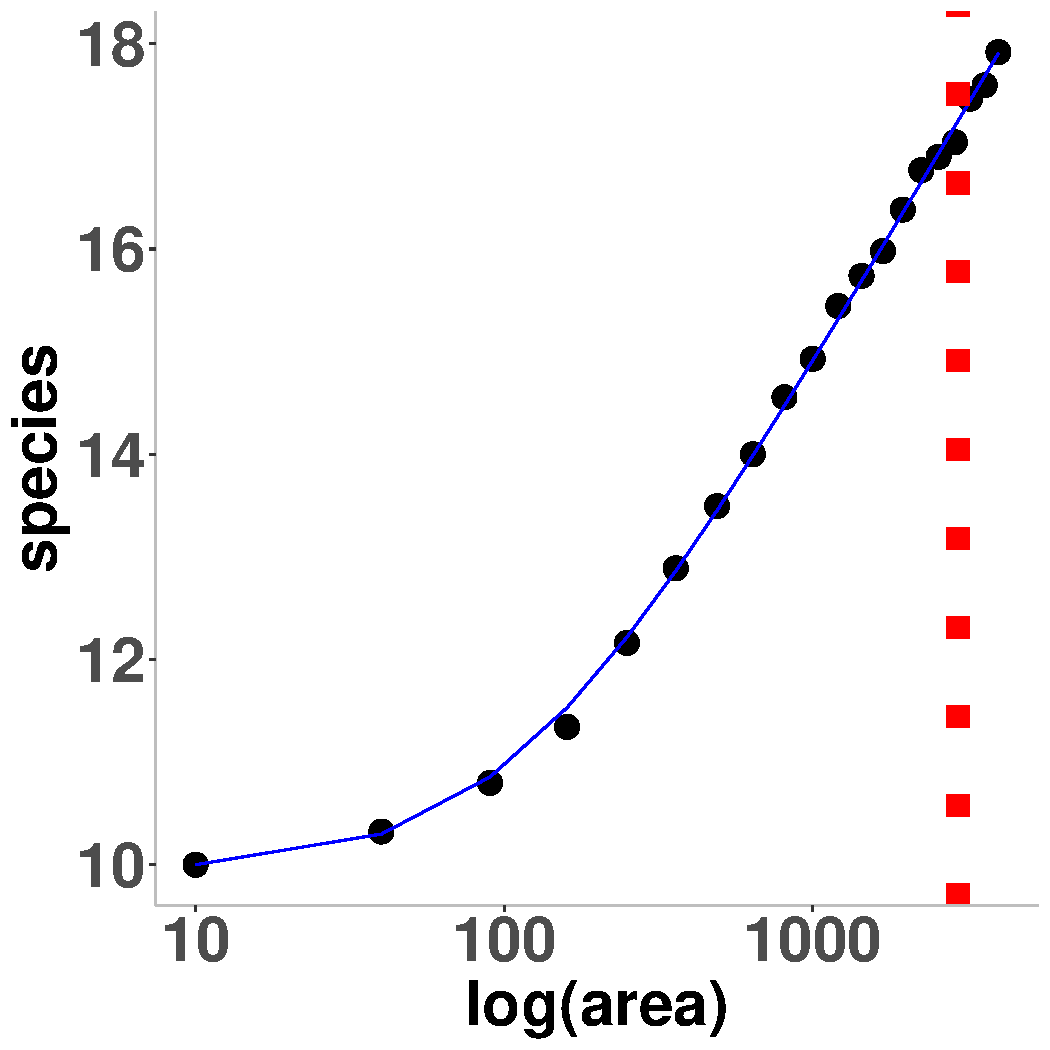
\includegraphics[width=0.3\linewidth]{../Results/Simulation/NLLSPlotClassic2.pdf}}
\subfloat[The Depth Model]{\label{fig:b}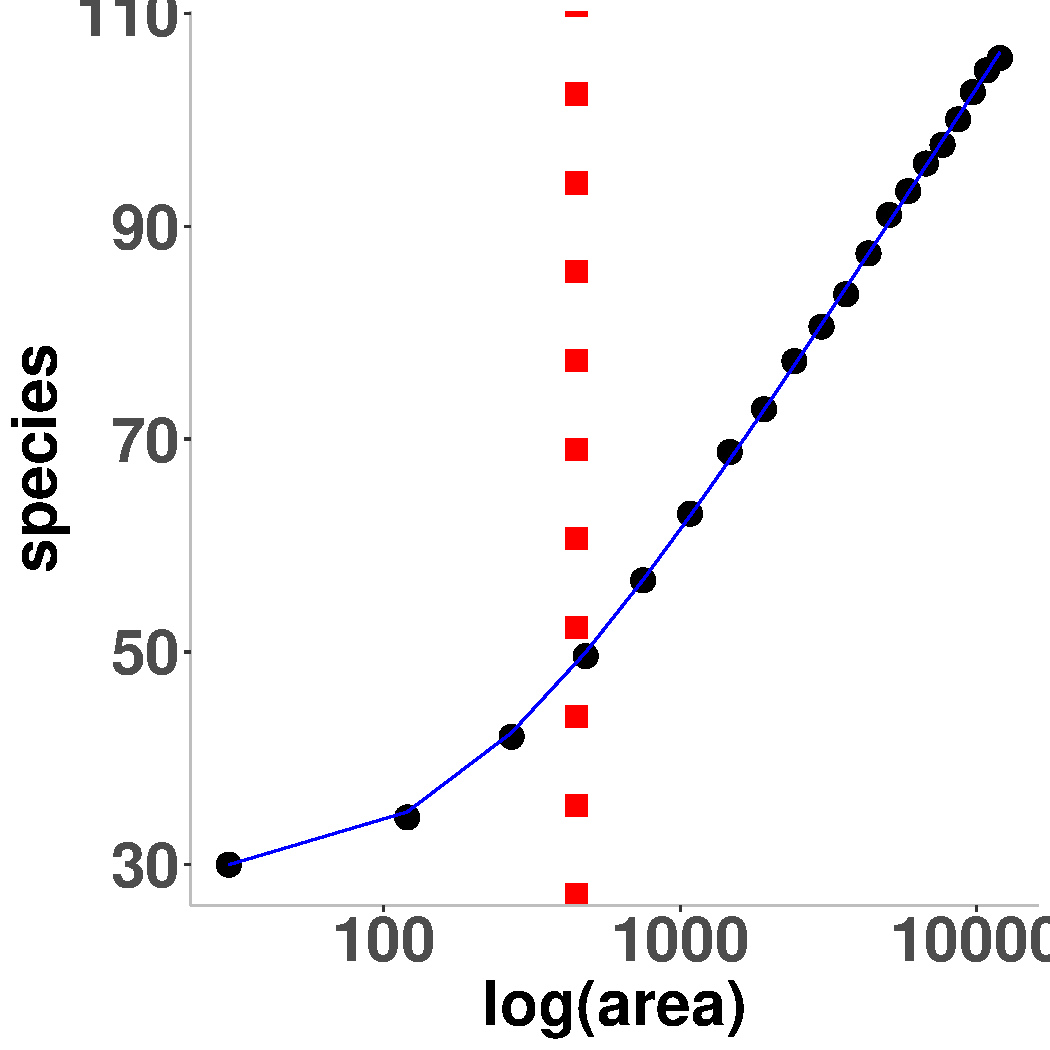
\includegraphics[width=0.3\linewidth]{../Results/Simulation/NLLSPlotDepth6.pdf}}
\subfloat[The Perimeter Model]{\label{fig:c}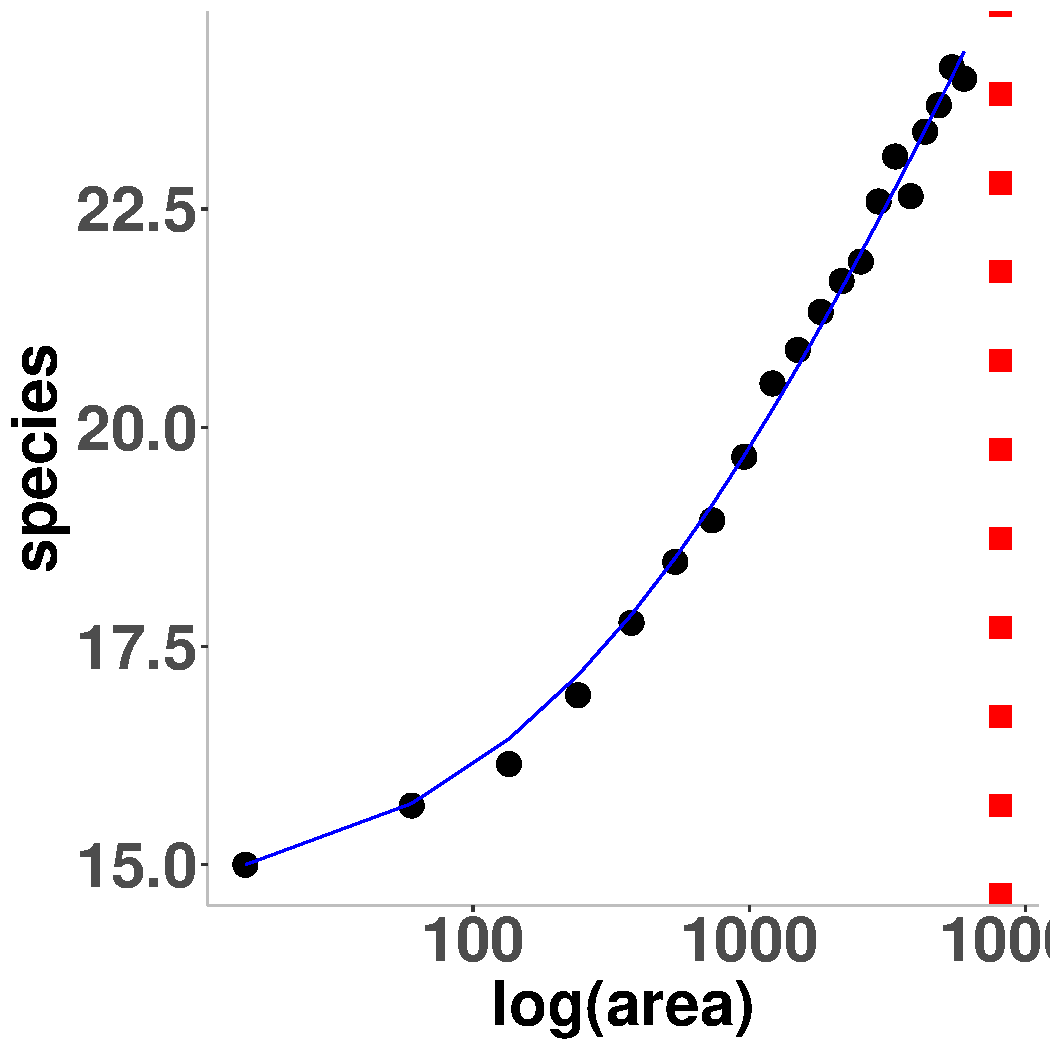
\includegraphics[width=0.3\textwidth]{../Results/Simulation/NLLSPlotPeri3.pdf}}
\smallskip


\includegraphics[width=.7\textwidth]{Legend.png}\\
\caption{NLLS fitting of the the simulation data. A) The Classic Model with true parameters $\theta$=20, \textit{m\textsubscript{0}}=0.2, \textit{K}=10 and estimated parameters $\theta$=20, \textit{m\textsubscript{0}}=0.2, \textit{K}=10. B) The Depth Model with true parameters $\theta$=18, \textit{m\textsubscript{0}}=0.06, \textit{K}=30 and estimated parameters $\theta$=19, \textit{m\textsubscript{0}}=0.05, \textit{K}=30. C) The Perimeters Model with true parameters $\theta$=30, \textit{m\textsubscript{0}}=0.5, \textit{K}=15 and estimated parameters $\theta$=57, \textit{m\textsubscript{0}}=0.46, \textit{K}=15.}
\label{fig:myfig}
\end{figure}

\noindent My results verified that the simulation and analytic formula are in agreement as expected. The three critical area formulas (see Methods 2.8-2.10) for each of the three model variations (Classic, Depth, Perimeter) give reasonable estimations of critical area (log \textit{A\textsubscript{crit}}).

\subsection{Classic Model}

\noindent The Classic Model fitting procedure fitted the simulated data well. Estimated parameters were slightly higher than the true parameters for $\theta$ and slightly lower for \textit{m\textsubscript{0}} and \textit{K}. There was a significant difference between the true and estimated values for $\theta$ (p=0.0008, 9 df) and \textit{m\textsubscript{0}} (p=0.0003, 9 df). There was no significant differences in true and estimated parameters for \textit{K} (p=0.34, 9 df).  As \textit{K} true and estimated parameters showed no significant difference, and there was only a small difference between \textit{m\textsubscript{0}} and $\theta$ true and estimated parameters, the model fitting process is considered validated and fit for applying to the empirical datasets.   \\

% From simulation on Thursday 13th August with J_meta 1,000,000, 20 islands, nu = 0.00001-0.0001, niches 5-50

\begin{figure}[htbp]
\centering
\subfloat[$\theta$ values]{\label{fig:a}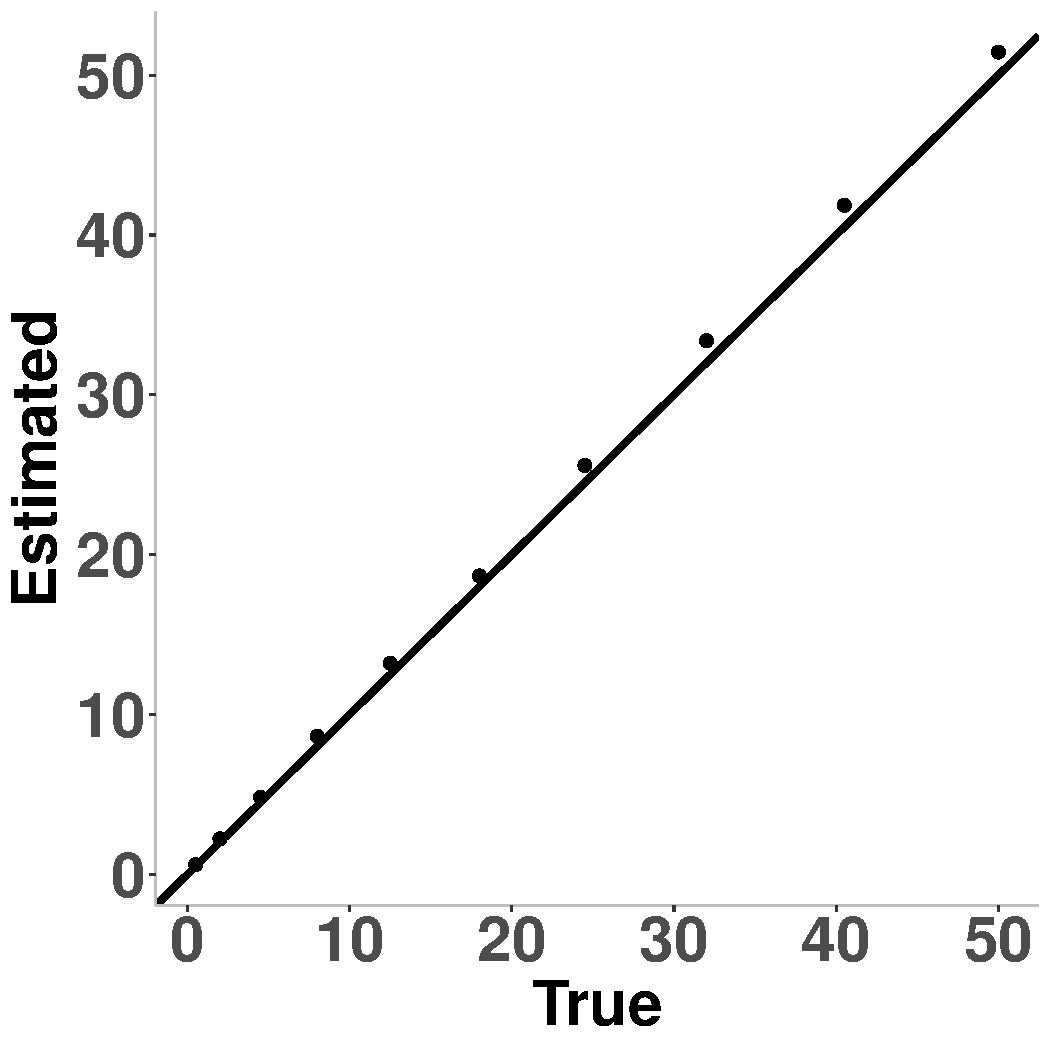
\includegraphics[width=0.3\linewidth]{AreaThetaResults.pdf}}
\subfloat[\textit{m\textsubscript{0}} values]{\label{fig:b}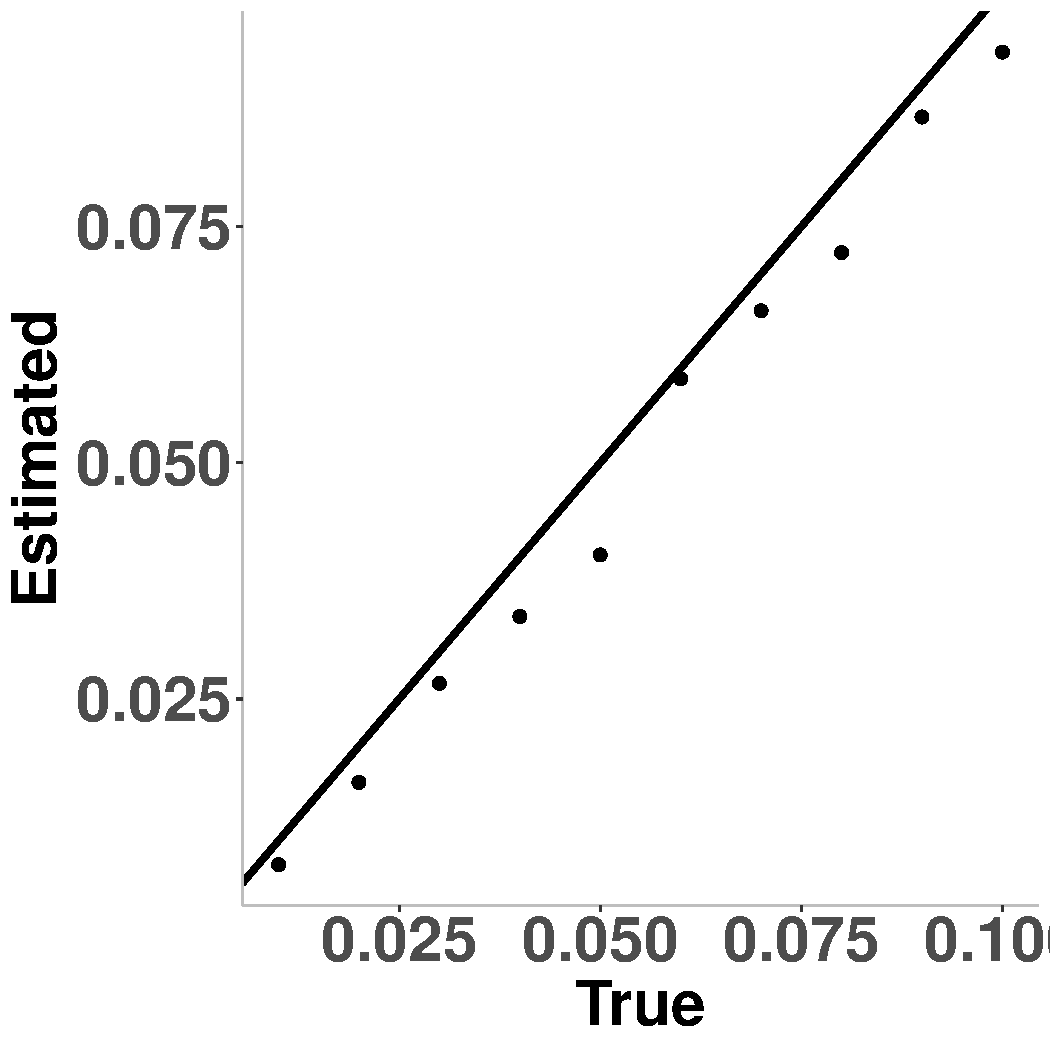
\includegraphics[width=0.3\linewidth]{Aream0Results.pdf}}
\subfloat[\textit{K} values]{\label{fig:c}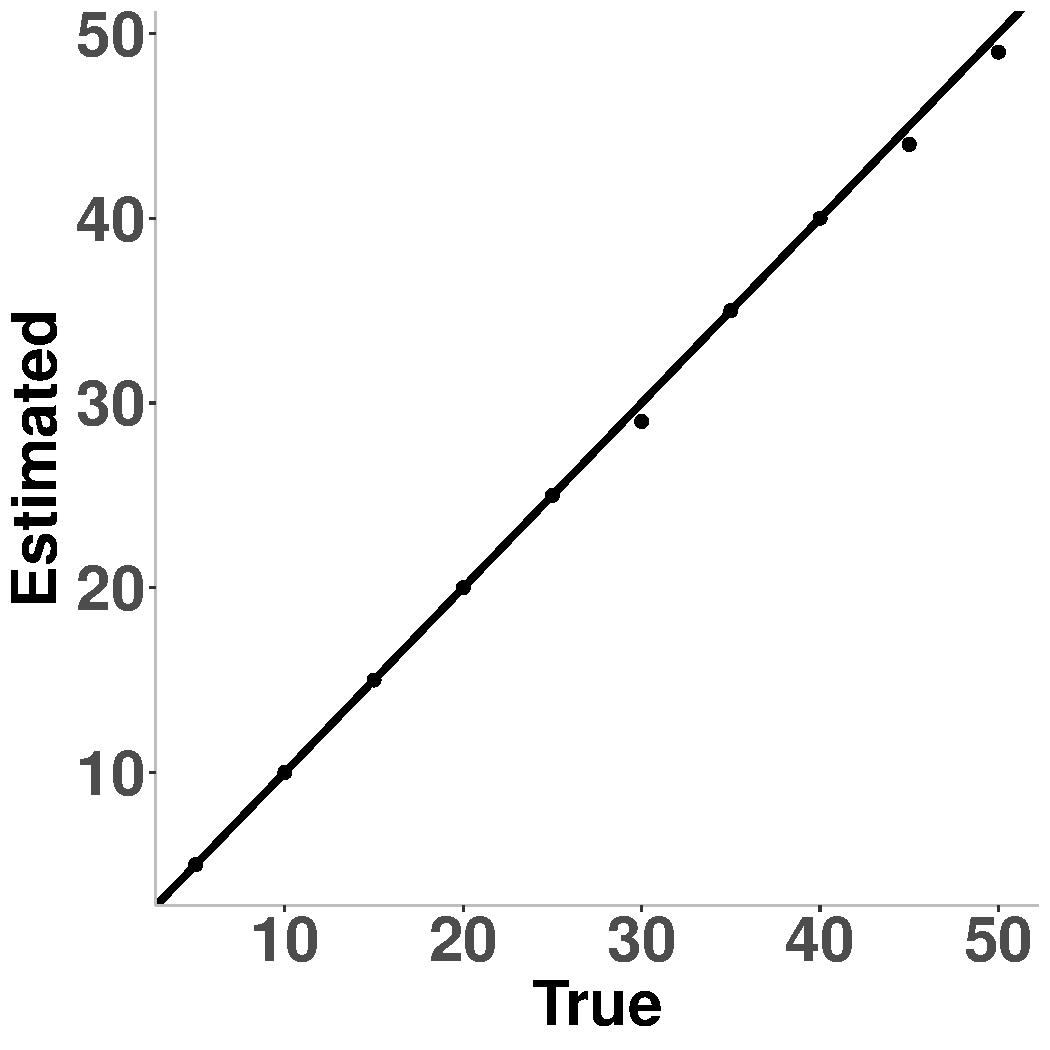
\includegraphics[width=0.3\textwidth]{AreaKResults.pdf}}
\smallskip


\includegraphics[width=.6\textwidth]{Legend2.png}\\
\caption{The true parameters values of $\theta$ (A), \textit{m\textsubscript{0}} (B) and \textit{K} (C) were simulated and the results fitted using the Classic Model analytical NLLS fitting procedure to get the parameters back. True and estimated values for the three fitted parameters are plotted above. Fittings of the Classic Model to simulated data returned mean R\textsuperscript{2} = 0.99, adjusted R\textsuperscript{2} = 0.99.}
\label{fig:myfig}
\end{figure}

\begin{table}[h!]
  \begin{center}
    \caption{Comparison between true and estimated mean parameters across 200 Area Model simulations clustered into 10 groups where parameter values ($\theta$, \textit{m\textsubscript{0}}, \textit{K}) were the same for each simulation group with varying areas.}
    \label{table5}
    \pgfplotstabletypeset[
      multicolumn names, % allows to have multicolumn names
      col sep=comma, % the seperator in our .csv file
      display columns/0/.style={
		column name=$Parameter$, % name of first column
		string type},  % use siunitx for formatting
      display columns/1/.style={
		column name=$True$,
		column type={S},string type},
      display columns/2/.style={
		column name=$Estimated$,
		column type={S},string type},
      display columns/3/.style={
		column name=$Difference$,
		column type={S},string type},
           every head row/.style={
		before row={\toprule}, % have a rule at top
		after row={
			%\si{\ampere} & \si{\volt}\\ % the units seperated by &
			\midrule} % rule under units
			},
		every last row/.style={after row=\bottomrule}, % rule at bottom
    ]{ClassicParam.csv} % filename/path to file
  \end{center}
\end{table}

%Mean RSquared result of fitting RSq 0.61
%Mean Adjusted RSquared 0.51

%What are the mean differences for each parameter? Positive or negative?
%theta = 2061.95 (estimation is 2061.95 scores higher), 
%m0 = -0.023 (estimation is -0.023 scores lower), 
%K = 0 (estimation is same as true values)

%Shapiro-Wilk Normality Test
%Are the differences normally distributed? 
%theta NO (W=0.77464, p=0.007123) 
%m0 YES (W=0.97794, p=0.9532) 

%Are the differences significant? 
%Wilcoxon signed rank test - because not normally distributed
%theta YES (V=1, p=0.0039) 

%Paired t-test
%m0 YES (t=4.0638, df=9, p=0.0028, CI 0.01039, 0.0365)



\subsection{Depth Model}

\noindent The Depth Model fitting procedure fitted the simulated data well. Estimated values of $\theta$ were higher, \textit{K} and  \textit{m\textsubscript{0}} values were lower than the true parameters (Table 3.2). There was a significant difference between the true and estimated values for $\theta$ (p=0.0005, 9 df) and \textit{m\textsubscript{0}} (p=0.005, 9 df), but there was no significant difference for \textit{K} (p=0.168, 9 df). As \textit{K} showed no significant difference, and the difference in estimated $\theta$ and \textit{m\textsubscript{0}} values was so low, the model fitting process is considered validated and fit for applying to the empirical datasets.  


% From simulation on Tuesday 11th August with J_meta 100000, 20 islands, nu = 0.0001-0.001, niches 5-50
%\hspace{10pt}\textbf{A} \hspace{135pt} \textbf{B} \hspace{130pt} \textbf{C}

\begin{figure}[htbp]
\centering
\subfloat[$\theta$ values]{\label{fig:a}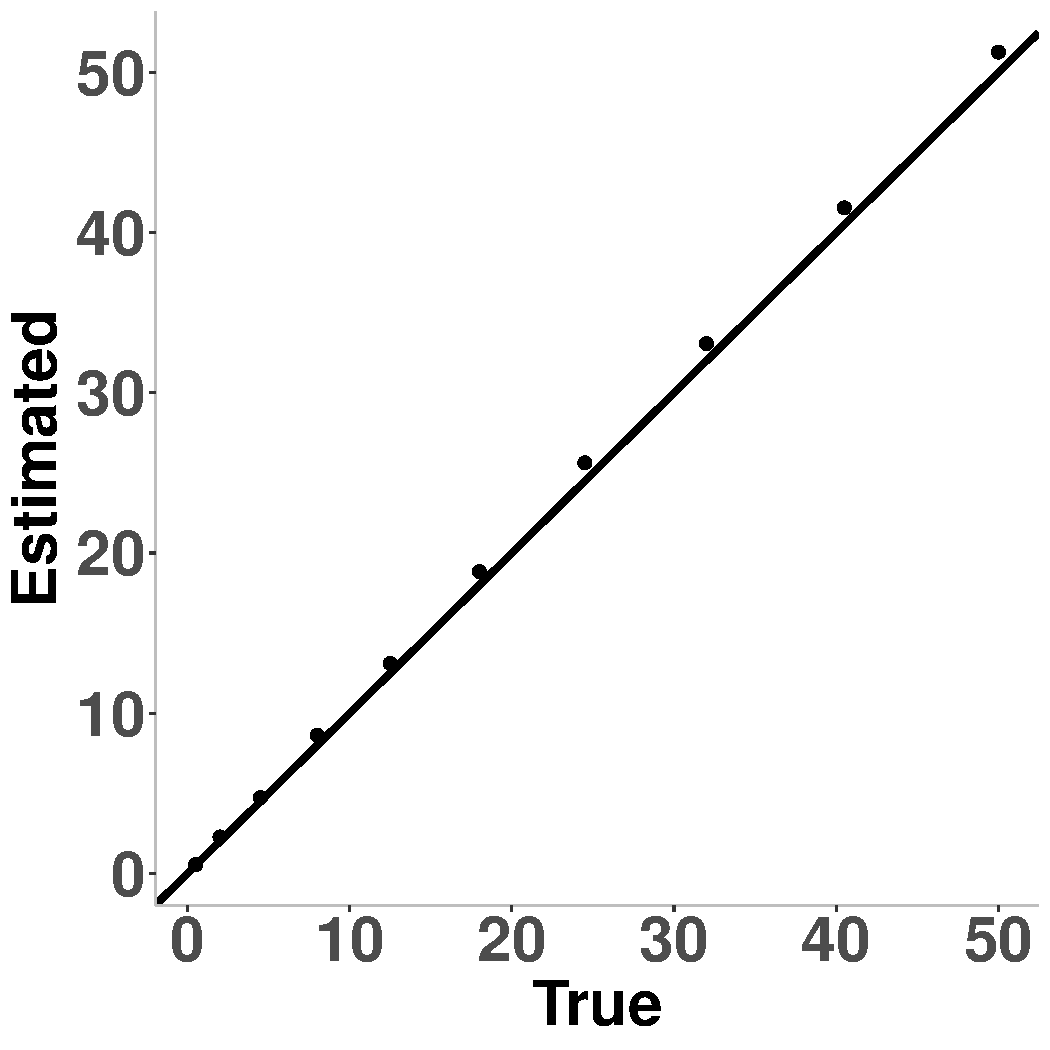
\includegraphics[width=0.3\linewidth]{DepthThetaResults.pdf}}
\subfloat[\textit{m\textsubscript{0}} values]{\label{fig:b}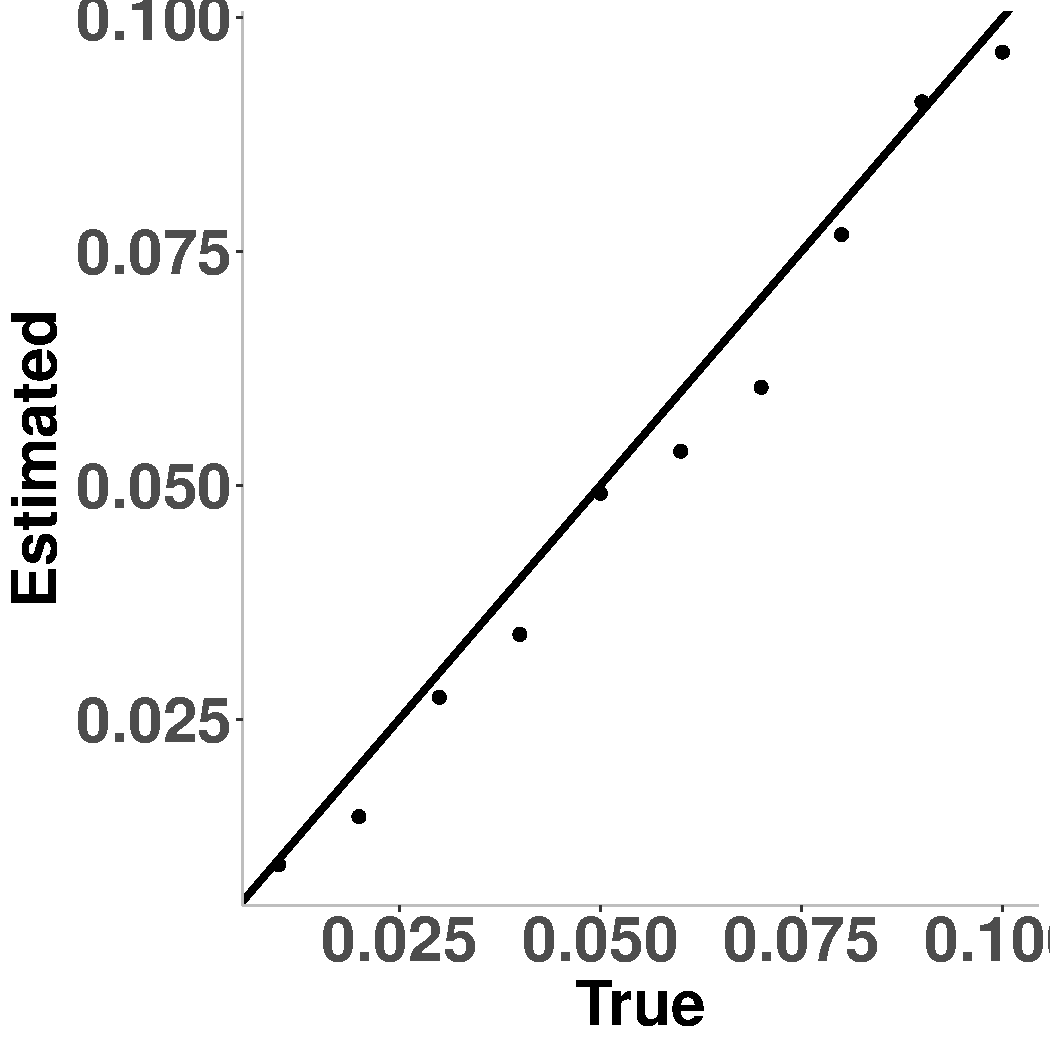
\includegraphics[width=0.3\linewidth]{Depthm0Results.pdf}}
\subfloat[\textit{K} values]{\label{fig:c}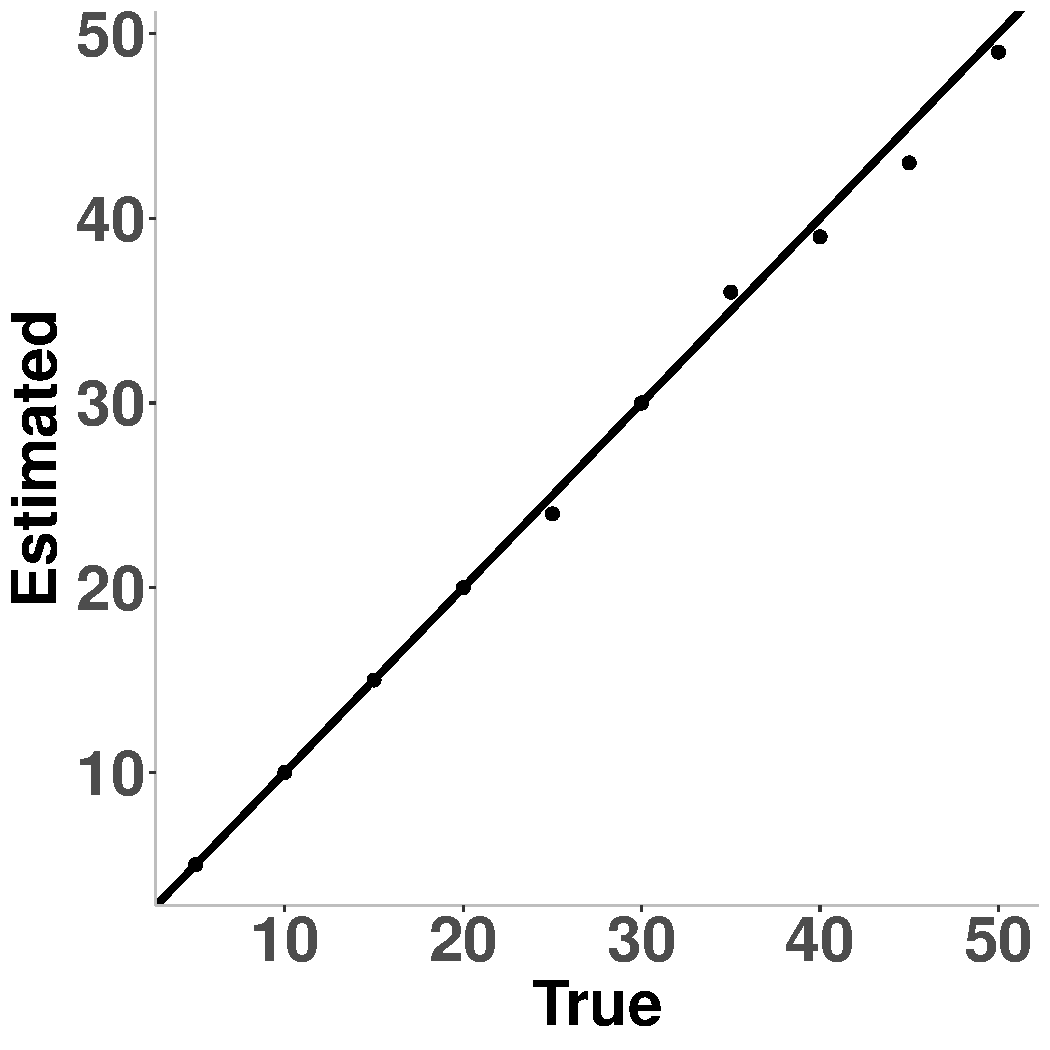
\includegraphics[width=0.3\textwidth]{DepthKResults.pdf}}
\smallskip


\includegraphics[width=.6\textwidth]{Legend2.png}\\
\caption{The true parameters values of $\theta$ (A), \textit{m\textsubscript{0}} (B) and \textit{K} (C) were simulated and the results fitted using the Depth Model analytical NLLS fitting procedure to get the parameters back. True and estimated values for the three fitted parameters are plotted above. Fittings of the Depth Model to simulated data returned mean R\textsuperscript{2} = 0.99, adjusted R\textsuperscript{2} = 0.99.}
\label{fig:myfig}
\end{figure}

\begin{table}[h!]
  \begin{center}
    \caption{Comparison between true and estimated mean parameters across 200 Depth Model simulations clustered into 10 groups where parameter values ($\theta$, \textit{m\textsubscript{0}}, \textit{K}) were the same for each simulation group with varying areas.}
    \label{table5}
    \pgfplotstabletypeset[
      multicolumn names, % allows to have multicolumn names
      col sep=comma, % the seperator in our .csv file
      display columns/0/.style={
		column name=$Parameter$, % name of first column
		string type},  % use siunitx for formatting
      display columns/1/.style={
		column name=$True$,
		column type={S},string type},
      display columns/2/.style={
		column name=$Estimated$,
		column type={S},string type},
      display columns/3/.style={
		column name=$Difference$,
		column type={S},string type},
           every head row/.style={
		before row={\toprule}, % have a rule at top
		after row={
			%\si{\ampere} & \si{\volt}\\ % the units seperated by &
			\midrule} % rule under units
			},
		every last row/.style={after row=\bottomrule}, % rule at bottom
    ]{DepthParam.csv} % filename/path to file
  \end{center}
\end{table} 


\subsection{Perimeter Model}


\begin{figure}[htbp]
\centering
\subfloat[$\theta$ values]{\label{fig:a}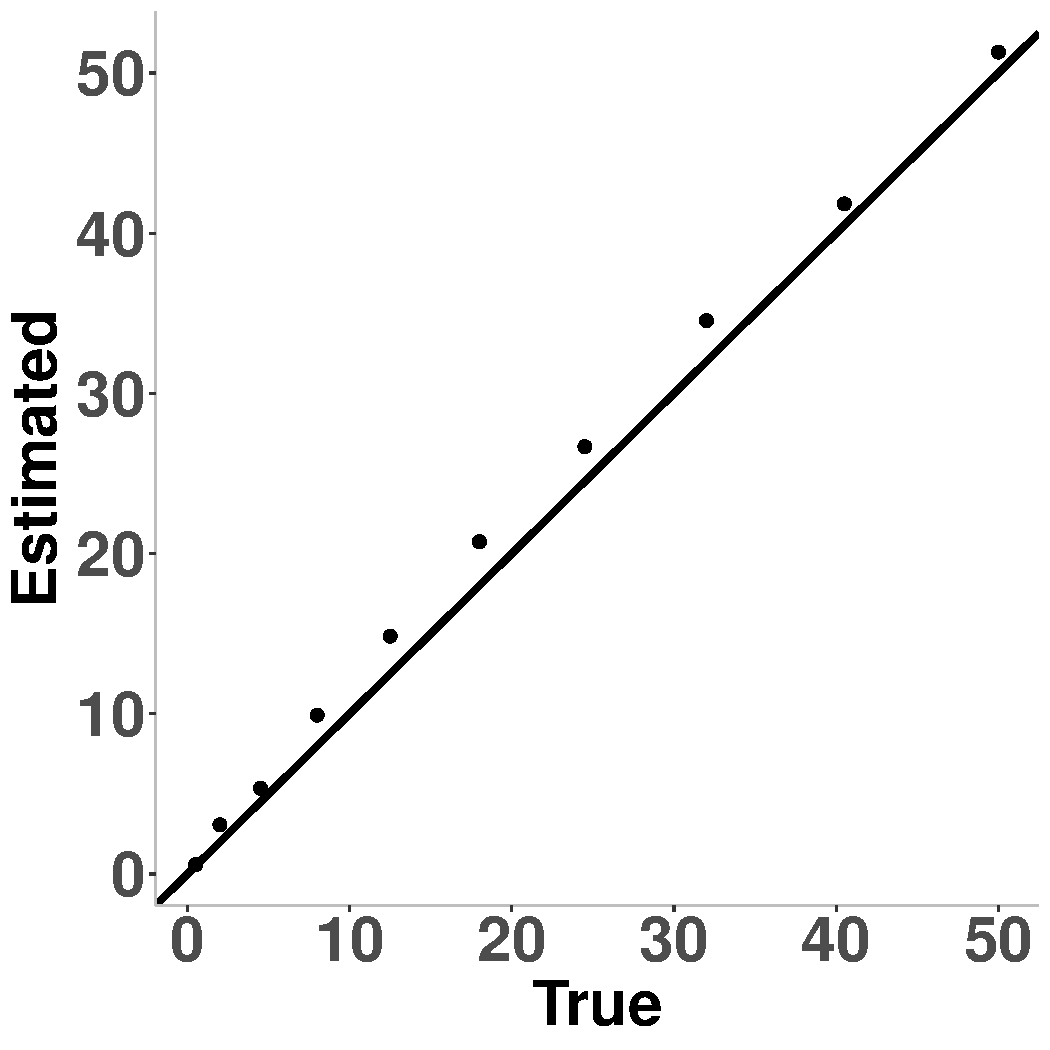
\includegraphics[width=0.3\linewidth]{PeriThetaResults.pdf}}
\subfloat[\textit{m\textsubscript{0}} values]{\label{fig:b}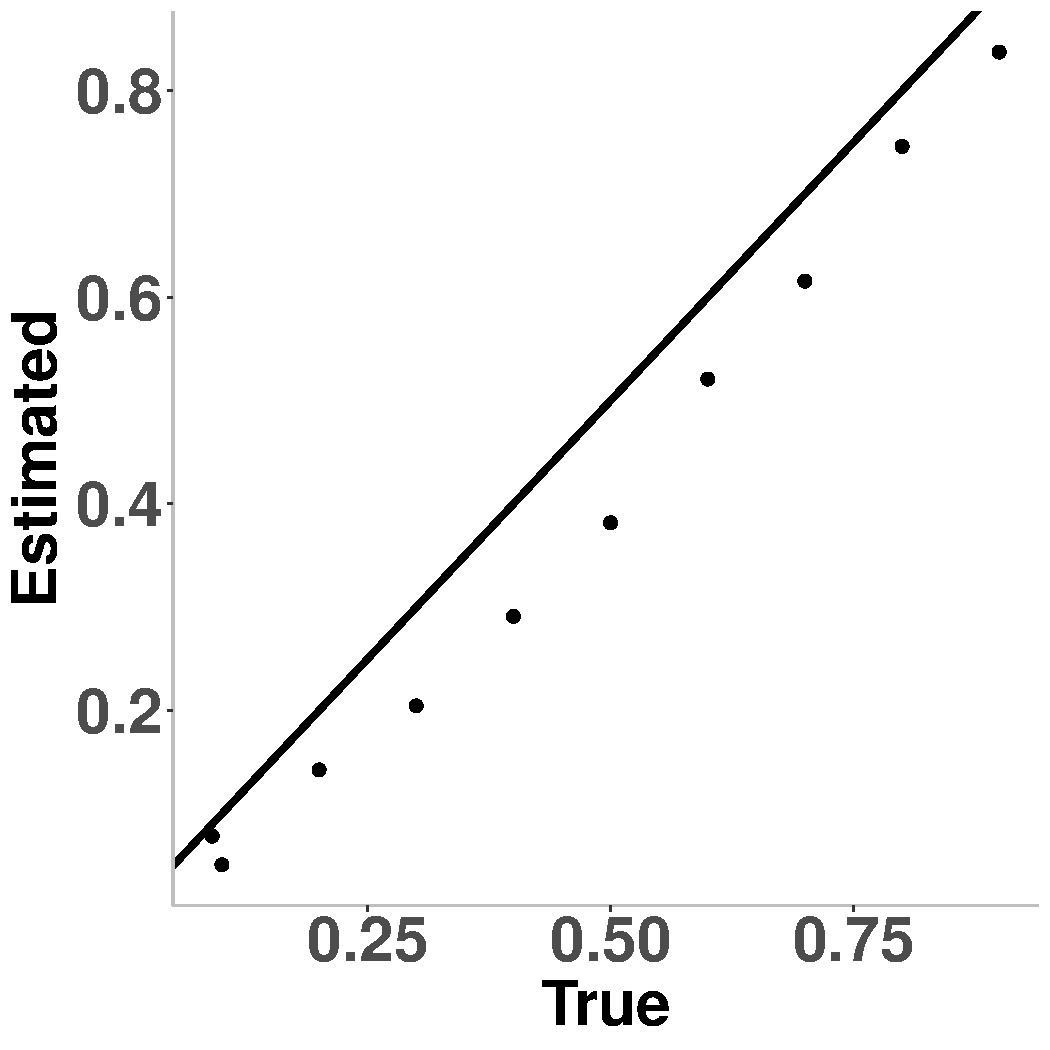
\includegraphics[width=0.3\linewidth]{Perim0Results.pdf}}
\subfloat[\textit{K} values]{\label{fig:c}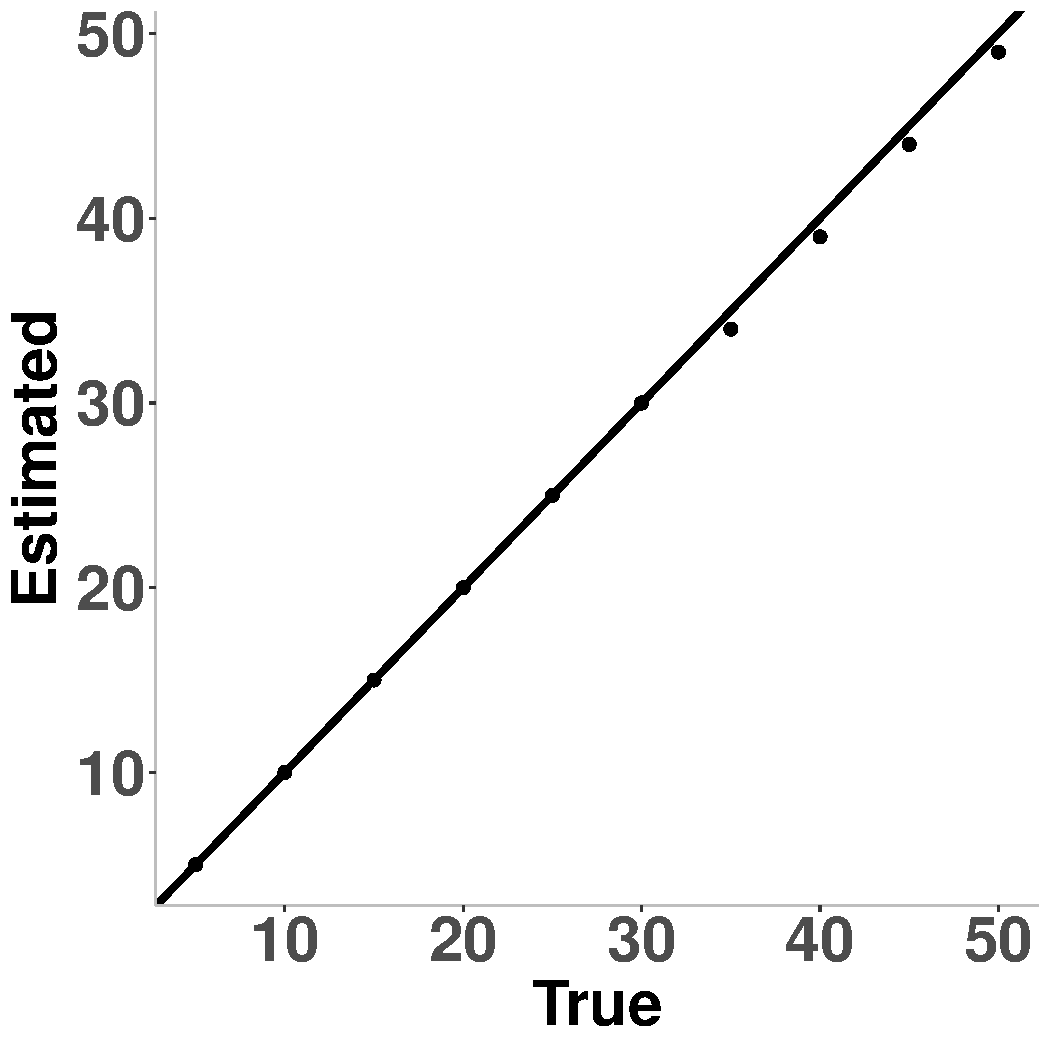
\includegraphics[width=0.3\textwidth]{PeriKResults.pdf}}
\smallskip


\includegraphics[width=.6\textwidth]{Legend2.png}\\
\caption{The true parameters values of $\theta$ (A), \textit{m\textsubscript{0}} (B) and \textit{K} (C) were simulated and the results fitted using the Perimeter Model analytical NLLS fitting procedure to get the parameters back. True and estimated values for the three fitted parameters are plotted above. Fittings of the Perimeter Model to simulated data returned mean R\textsuperscript{2} = 0.99, adjusted R\textsuperscript{2} = 0.99.}
\label{fig:myfig}
\end{figure}

\begin{table}[h!]
  \begin{center}
    \caption{Comparison between true and estimated mean parameters across 200 Perimeter Model simulations clustered into 10 groups where parameter values ($\theta$, \textit{m\textsubscript{0}}, \textit{K}) were the same for each simulation group with varying areas.}
    \label{table5}
    \pgfplotstabletypeset[
      multicolumn names, % allows to have multicolumn names
      col sep=comma, % the seperator in our .csv file
      display columns/0/.style={
		column name=$Parameter$, % name of first column
		string type},  % use siunitx for formatting
      display columns/1/.style={
		column name=$True$,
		column type={S},string type},
      display columns/2/.style={
		column name=$Estimated$,
		column type={S},string type},
      display columns/3/.style={
		column name=$Difference$,
		column type={S},string type},
           every head row/.style={
		before row={\toprule}, % have a rule at top
		after row={
			%\si{\ampere} & \si{\volt}\\ % the units seperated by &
			\midrule} % rule under units
			},
		every last row/.style={after row=\bottomrule}, % rule at bottom
    ]{PeriParam.csv} % filename/path to file
  \end{center}
\end{table}

\noindent The Perimeter Model fitting procedure fitted the simulated data well. Estimated parameters for $\theta$ were slightly higher than true parameters, whilst \textit{m\textsubscript{0}} and \textit{K} were slightly lower than the true parameters (Table 3.3). There was significant difference between the true and estimated values for $\theta$ (p=0.0002, 9 df), \textit{m\textsubscript{0}} (p=5x10\textsuperscript{5}, 9 df) and \textit{K} (p=0.04, 9df). Despite the significant difference between the estimated and true values for my simulation parameters, the differences are small enough that the model fitting process is considered validated and fit for applying to the empirical datasets.   

\section{Model Fitting}

%How many datasets did I start with?
%Are they all listed in the supplementary materials?

\subsection{Non-Linear Least Squares Fitting}


\noindent 50 of the 57 datasets exhibited a positive TAR and were used for the NLLS fitting. Of the 50 datasets fitted with the three models, 26 failed to achieve adjusted R\textsuperscript{2} scores of between 0 and 1. These datasets were excluded from further analysis (see Supplementary Materials, Figure 7.2). 

\begin{table}[h!]
  \begin{center}
    \caption{The mean R\textsuperscript{2} and adjusted R\textsuperscript{2} results for each model (Classic, Depth, Perimeter) after being successfully fitted to 26 empirical datasets.}
    \label{table5}
    \pgfplotstabletypeset[
      multicolumn names, % allows to have multicolumn names
      col sep=comma, % the seperator in our .csv file
      display columns/0/.style={
		column name=$Model$, % name of first column
		string type},  % use siunitx for formatting
      display columns/1/.style={
		column name=$R\textsuperscript{2}$,
		column type={S},string type},
      display columns/2/.style={
		column name=$Adj R\textsuperscript{2}$,
		column type={S},string type},
           every head row/.style={
		before row={\toprule}, % have a rule at top
		after row={
			%\si{\ampere} & \si{\volt}\\ % the units seperated by &
			\midrule} % rule under units
			},
		every last row/.style={after row=\bottomrule}, % rule at bottom
    ]{RResults.csv} % filename/path to file
  \end{center}
\end{table}

\noindent All three models had similar mean R\textsuperscript{2} and adjusted R\textsuperscript{2} scores and total results show the models fit the data moderately well (Table 3.4). The Classic Model was best-fit for 1 dataset, Depth and Perimeter were best for 2 each and the rest of the datasets were either best described by both Classic and Depth or all of the models (Table 3.5). The differences in R\textsuperscript{2} scores for each of the fittings was small (see Supplementary Materials, Table 7.5). For datasets that were equally well fit to two or more of the models I found the mean \textit{A\textsubscript{crit}} and parameter estimations ($\theta$, \textit{m\textsubscript{0}}, \textit{K}) for each of those fittings and used these in the proceeding analysis. \\

\begin{table}[h!]
  \begin{center}
    \caption{The best-fit models (Classic, Depth, Perimeter) by highest adjusted R\textsuperscript{2} value for each empirical dataset (note some datasets had equal adjusted R\textsuperscript{2} values for two or more models). }
    \label{table5}
    \pgfplotstabletypeset[
      multicolumn names, % allows to have multicolumn names
      col sep=comma, % the seperator in our .csv file
      display columns/0/.style={
		column name=$Models$, % name of first column
		string type},  % use siunitx for formatting
      display columns/1/.style={
		column name=$Best Fit$,
		column type={S},string type},
           every head row/.style={
		before row={\toprule}, % have a rule at top
		after row={
			%\si{\ampere} & \si{\volt}\\ % the units seperated by &
			\midrule} % rule under units
			},
		every last row/.style={after row=\bottomrule}, % rule at bottom
    ]{BestModel.csv} % filename/path to file
  \end{center}
\end{table}

\noindent The best model fits had mean R\textsuperscript{2} = 0.49 and mean adjusted R\textsuperscript{2} = 0.41 with standard deviation 0.28 and range 0.01 - 0.96. The median value of $\theta$ was 8, with a range of 0.28 -- 159709. The median value of \textit{m\textsubscript{0}} was 2.17 x10\textsuperscript{-9} with a range of 4.97 x 10\textsuperscript{-16} -- 0.56. The median value for \textit{K} was 7, with range 1 -- 424. There was no correlation detected between the best fitted-values of the four parameters (Table 3.6). \\

\begin{table}[h!]
  \begin{center}
    \caption{p-values of correlations between the four model parameters ($\theta$, \textit{m\textsubscript{0}}, \textit{K}, $\rho$) that show no correlation}
    \label{table5}
    \pgfplotstabletypeset[
      multicolumn names, % allows to have multicolumn names
      col sep=comma, % the seperator in our .csv file
      display columns/0/.style={
		column name=$Parameter$, % name of first column
		string type},  % use siunitx for formatting
      display columns/1/.style={
		column name=$K$,
		column type={S},string type},
      display columns/2/.style={
		column name=$Theta$,
		column type={S},string type},
        display columns/3/.style={
		column name=$m\textsubscript{0}$,
		column type={S},string type},
	 display columns/4/.style={
		column name=$rho$,
		column type={S},string type},
           every head row/.style={
		before row={\toprule}, % have a rule at top
		after row={
			%\si{\ampere} & \si{\volt}\\ % the units seperated by &
			\midrule} % rule under units
			},
		every last row/.style={after row=\bottomrule}, % rule at bottom
    ]{Spearmansrank_p_corr.csv} % filename/path to file
  \end{center}
\end{table}

%How often was the power-law model a better fit to the data than the three models?
\noindent Mean \textit{z} value for the 50 datasets (prior to removing failed fits) was 0.16. The power-law model had the same number of successful fittings as the Classic, Depth and Perimeter models. After removing failed fits the mean \textit{z} value remained the same. The power-law model performed slightly more poorly than the other three models (R\textsubscript{2}=0.47, adjusted R\textsubscript{2}=0.38) (see Supplementary Materials, Table 7.3). AIC scores indicated that the power-law model was not a more parsimonious model than the Classic, Depth or Perimeter models relative to model fit for any of the 24 successfully fitted datasets (see Supplementary Materials, Table 7.4). The Classic and Depth models were significantly better than the power-law model for 9 datasets each. The Perimeter model was a better fit than the power-law model for 5 datasets.   
  
\section{Critical Area}
{\texorpdfstring
Off the five habitat types (terrestrial, riverine, lacustrine, plant and machine) and six taxonomic groups (algae, archaea, bacteria, fungi, pathogens and protozoa), the riverine habitat and archaea group did not have any successful fittings and are excluded from the following analysis.\\


\begin{figure}[htbp]
\centering
\subfloat[Dataset 45, bacteria in biomembrane reactors]{\label{fig:a}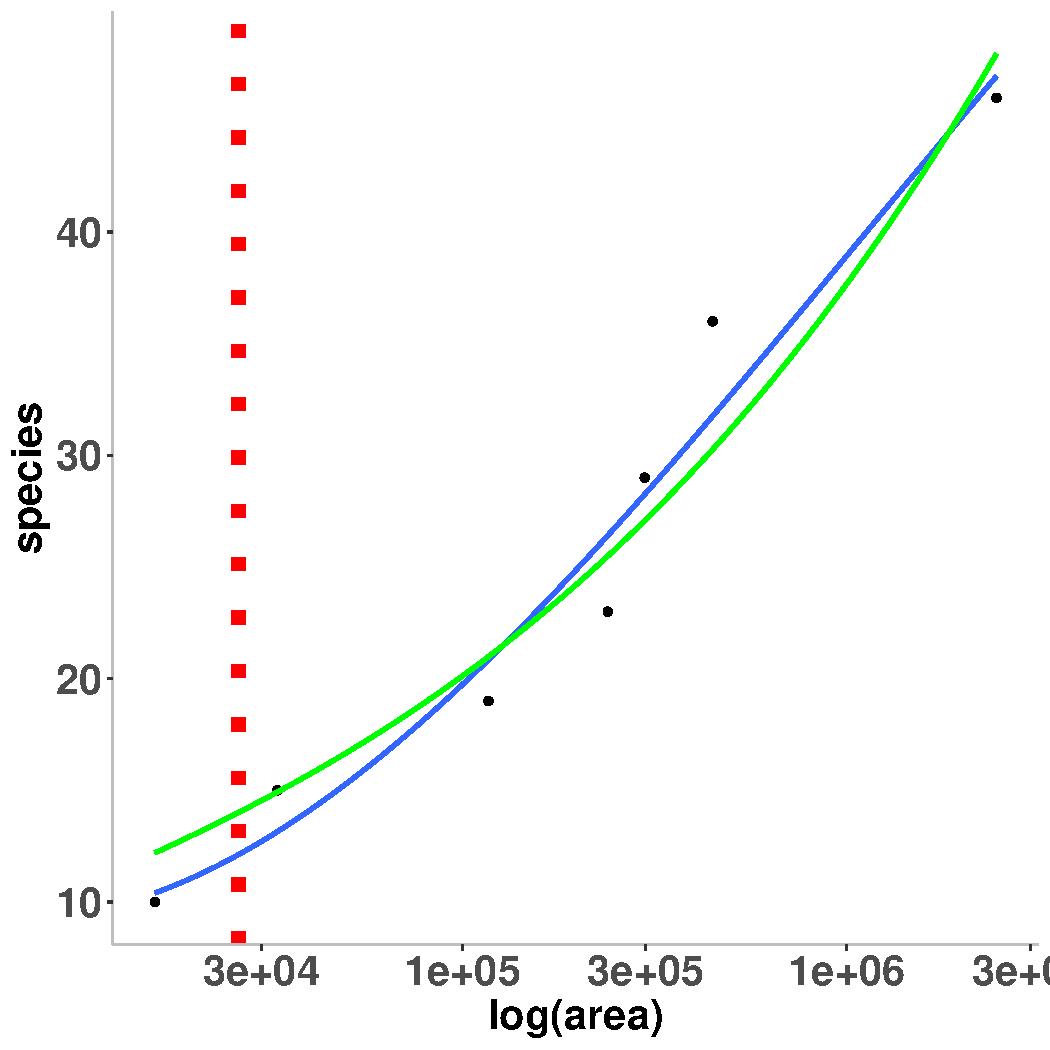
\includegraphics[width=0.45\linewidth]{../Results/ClassicNLLSPlot39.pdf}}\qquad
\subfloat[Dataset 44, fungi in plant root soil]{\label{fig:b}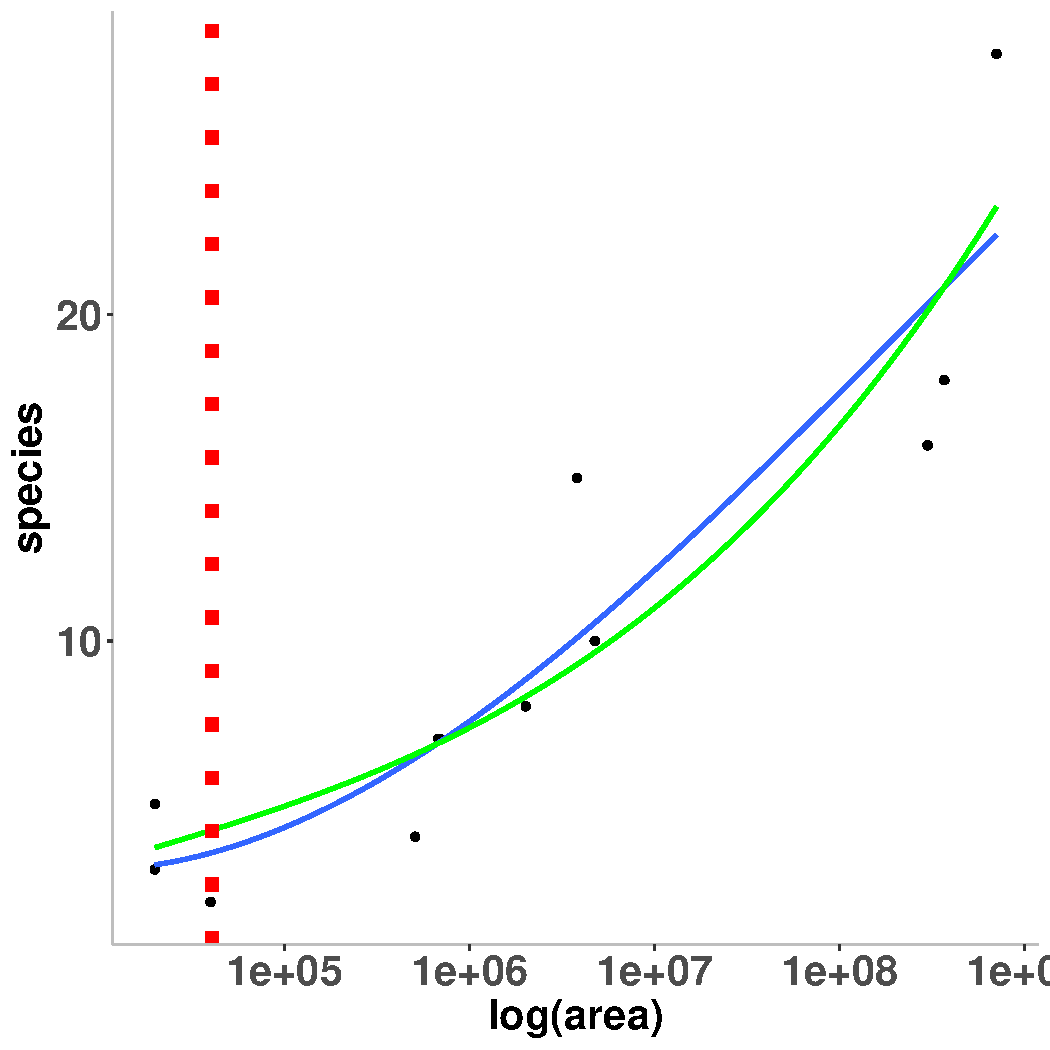
\includegraphics[width=0.45\linewidth]{../Results/PeriNLLSPlot38.pdf}}\\
\subfloat[Dataset 46, bacteria in tree holes (log area plotted with depth)]{\label{fig:c}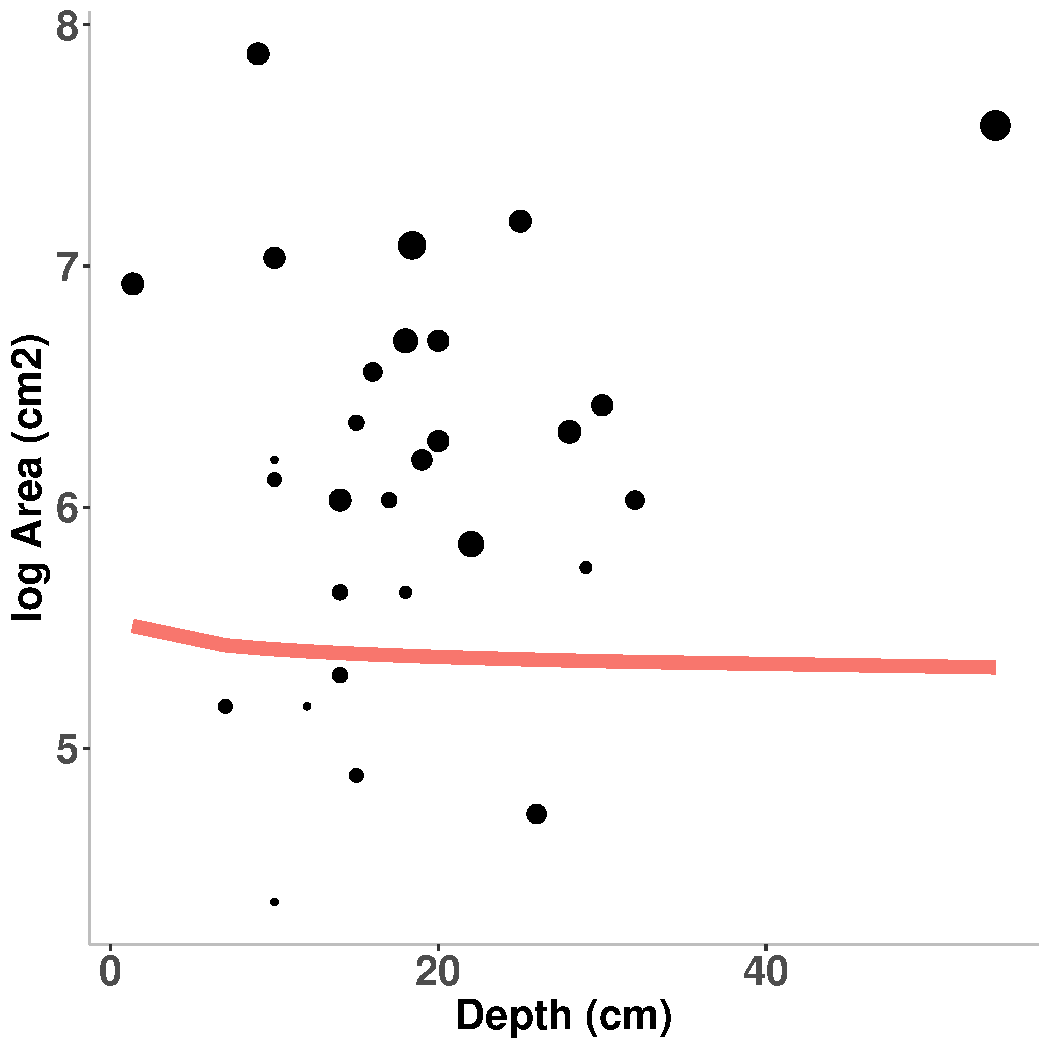
\includegraphics[width=0.45\textwidth]{../Results/DepthNLLSPlot40.pdf}}\qquad%
\subfloat[Dataset 46, bacteria in tree holes (log volume plotted with OTU richness)]{\label{fig:d}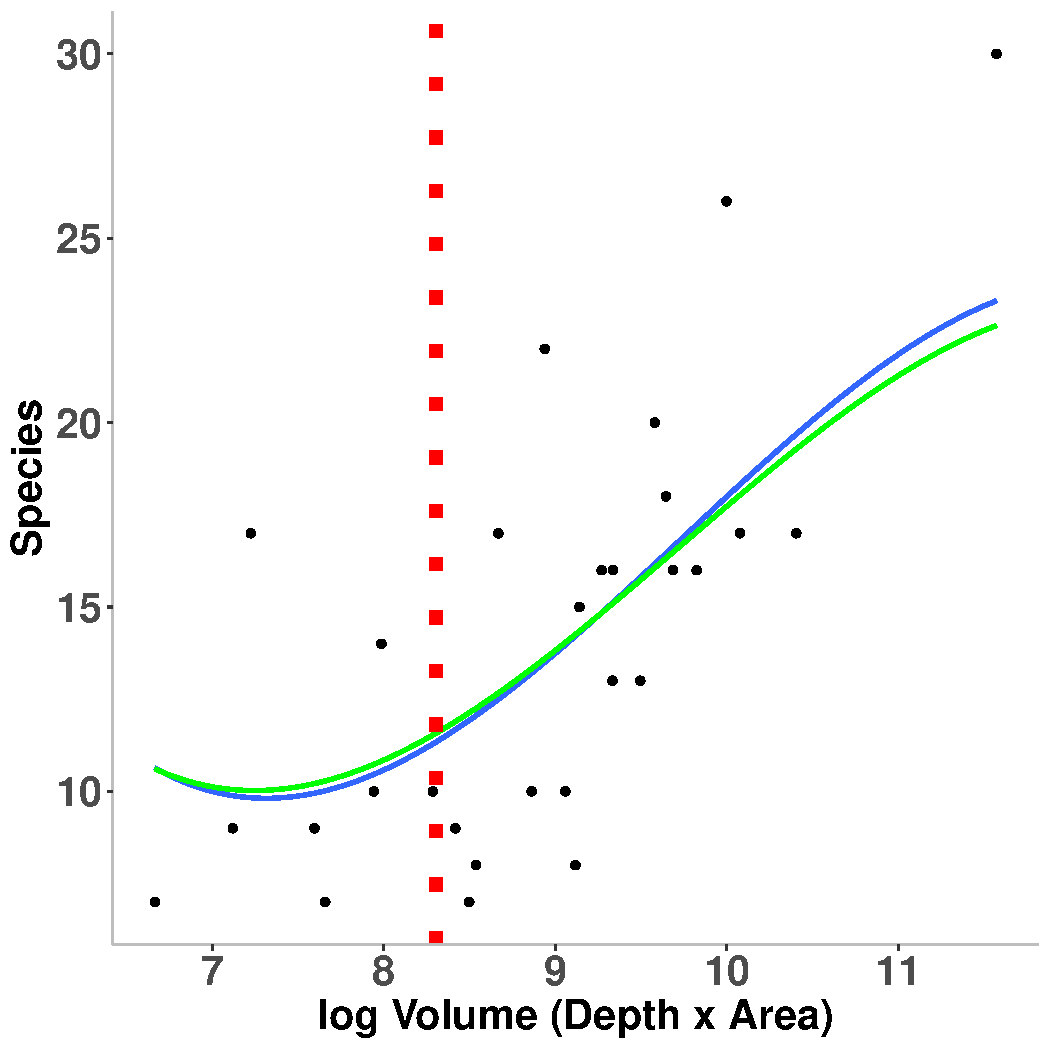
\includegraphics[width=0.45\textwidth]{../Results/DepthNLLSPlot2_40.pdf}}%
\caption{A) Best-fit Classic Model for dataset 45, bacteria in biomembrane reactors. Red line indicates \textit{A\textsubscript{crit}}, blue line indicates NLLS fit and green line indicates power-law fit (R\textsuperscript{2}=0.96, adjusted R\textsuperscript{2}=0.88, $\theta$=9, \textit{m\textsubscript{0}}=4.97 x 10\textsuperscript{-16}, \textit{K}=7). B) Best-fit Perimeter Model for dataset 44, fungi in plant soil (R\textsuperscript{2}=0.85, adjusted R\textsuperscript{2}=0.77, $\theta$=5, \textit{m\textsubscript{0}}=6.15 x 10\textsuperscript{-11}, \textit{K}=2). C) Best-fit Depth Model for dataset 46, bacteria in freshwater treeholes. The size of the black circles represents increasing OTU richness at that corresponding depth (x-axis) and log area (y axis) (R\textsuperscript{2}=49, adjusted R\textsuperscript{2}=0.40, $\theta$=8, \textit{m\textsubscript{0}}=3.75 x 10\textsuperscript{-9}, \textit{K}=6). Where the red line passes through depth and area space is where \textit{A\textsubscript{crit}} occurs. D) Dataset 46 plotted as log Volume by OTU richness to illustrate the model fit and log critical volume (A\textsubscript{vol})}
\label{fig:myfig}
\end{figure}

\noindent The log \textit{A\textsubscript{crit}} data were not normally distributed with non-homogenous variances. Despite the violation of normality I have proceeded with the multiple regression analysis, although interpretation of results will take this into consideration. \\

\noindent Initial multiple regression revealed that the model was a poor fit to the data (R\textsuperscript{2}=0.39, adjusted R\textsuperscript{2}=0.05, p=0.374) and neither categorical variable was significant in predicting log \textit{A\textsubscript{crit}} (habitat type p=0.1759, taxonomic group p=0.6402). A plot of the model indicated that there was an outlying data point. After removing the outlying data point the model was significant in describing the data (R\textsuperscript{2}=0.62, adjusted R\textsuperscript{2}=0.44, p=0.02). Taxonomic group became weakly significant in predicting log \textit{A\textsubscript{crit}} (p=0.0187) but habitat type did not (p=0.097). After removing habitat type as a categorical dependent variable the model was a similar fit to the data but more significant (R\textsuperscript{2}=0.55, adjusted R\textsuperscript{2}=0.45, p=0.004).\\

\noindent Multiple regression including taxonomic group only upheld the prediction that \textit{A\textsubscript{crit}} would occur at lower areas for more motile OTUs as bacteria show the lowest log\textit{A\textsubscript{crit}} estimate and host-dependent pathogens show the highest (Table 3.7). \\

\noindent There was a large variation in mean log \textit{A\textsubscript{crit}} between habitats and taxonomic groups. Terrestrial habitats showed the highest mean log \textit{A\textsubscript{crit}} (27.33), whilst machine habitats showed the lowest (4.66) (Figure 3.6). Pathogens exhibited the largest mean \textit{A\textsubscript{crit}} for taxonomic groups (55.15), with bacteria having the lowest (4.06) (Figure 3.6). \\

\begin{figure}[htp]

\centering
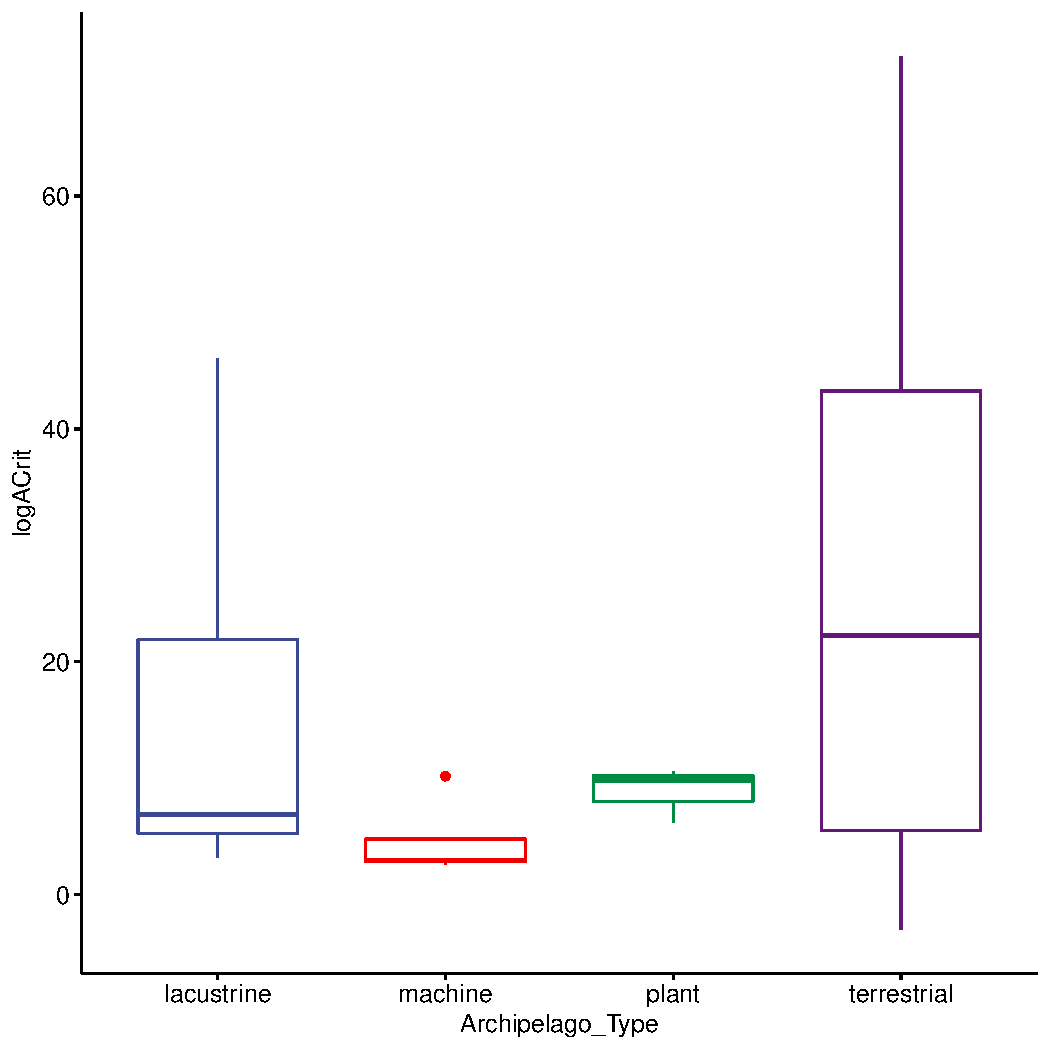
\includegraphics[width=.5\textwidth]{BoxplotTotalACritArch.pdf}\hfill
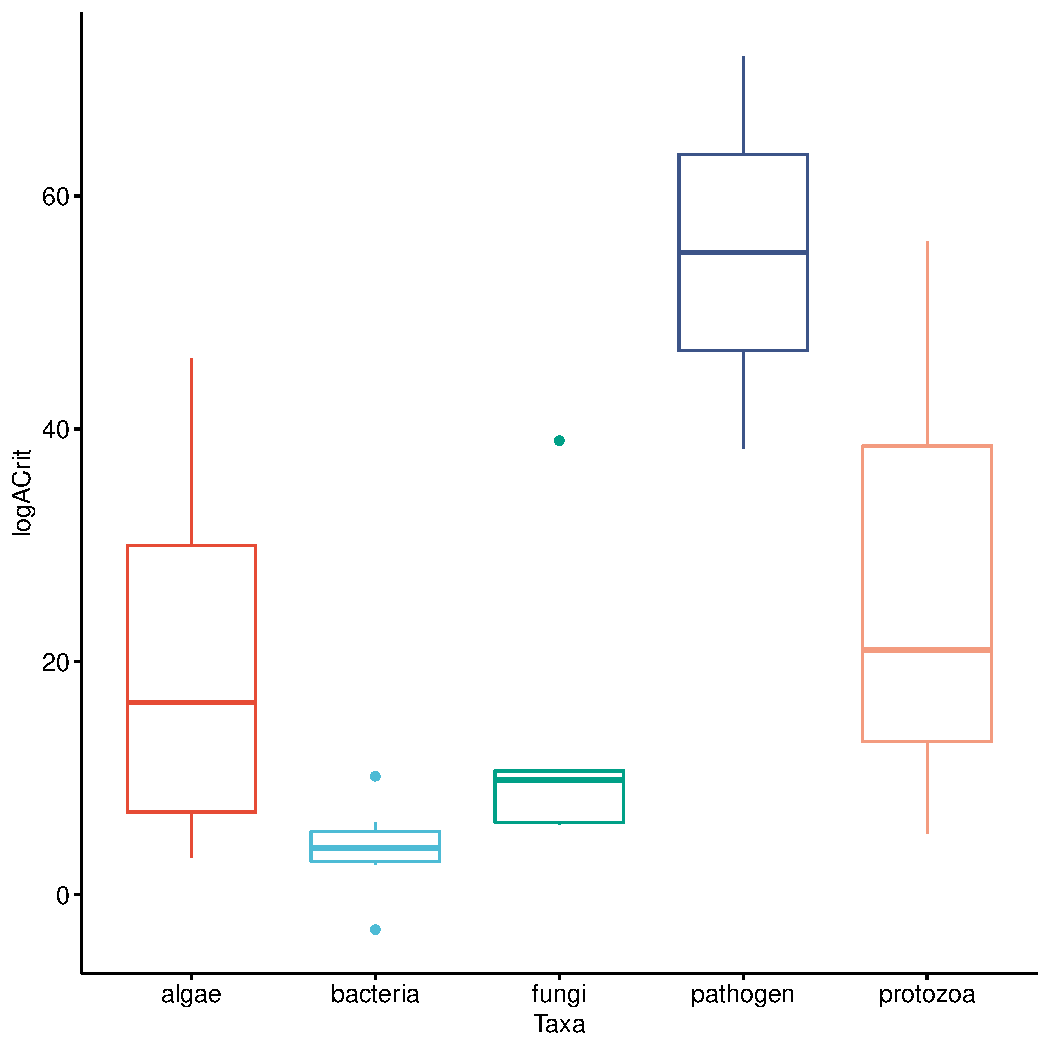
\includegraphics[width=.5\textwidth]{BoxplotTotalACritTaxa.pdf}\hfill

\hspace{10pt}\textbf{Habitat Type} \hspace{110pt} \textbf{Taxonomic Group}

\caption{log \textit{A\textsubscript{crit}} by habitat type and taxonomic group after removing anomalous result}
\label{fig:figure8}

\end{figure}



\noindent    


%Shapiro test for normality indicates logACrit is NOT normally distributed
%Both habitat type and taxa has non-homogenous variances 
%I have continued with the ANOVA and regression analysis but will keep in mind the 
%large variances within the data
%The assumptions of normality were violated as the ratio of variance between the largest log(ACrit) habitat type variance was 800 times larger than the smallest variance.
%The assumptions of normality were violated as the ratio of the variance between largest log(ACrit) taxa variance was 5 times larger than the smallest variance.
%Visual inspection of a histogram of log(ACrit) values indicated they were not normally distributed
%There does appear to be a large number of lower values in the histogram.
%After running an ANOVA of a linear model of logACrit with Habitat type and taxa group as categorical explainatory variables, I divided the mean square variation for each variable by the residual mean square variation. This indicated that habitat type (935.3728/349.1180 = 2.679246) was more important in influencing logACrit than taxa group (424.1640/349.1180 = 1.214959). 
%summary of my model indicated that none of the estimated mean differences for habitat type vary from the first(lacustrine) and non of the estimated mean differences for taxa group differ from the first (algae).
%The model is poor at explaining the data 
%A Tukey test indicated that none of the habitat types or taxa groups were significant in predicting logACrit.
%A plot of the model indicated that it could not be validated and there were three outlying datapoints (particularly point 21)
%This point was removed and the model re-run

%\noindent A Shapiro test for normality indicated that log ACrit values were not normally distributed, with habitat type and taxonomic group exhibiting non-homogenous variances. The assumptions of normality were violated for habitat type and taxonomic group and this was confirmed by visual inspection of histograms. Despite this I have proceeded with the multiple regression analysis, although interpretation of results will take this into consideration. \\

%\noindent A multiple regression (two-way ANOVA) was run with log ACrit as dependent variable and habitat type and taxonomic group as independent categorical variables. I divided the mean square variation for each independent variable by the residual mean square variation to find the relative influence of habitat type and taxonomic group on log ACrit. The results indicated that habitat type (1282.40/743.24 = 1.73) was more important in influencing log ACrit than taxa group (489.84/743.24 = 0.66). The model was poor at explaining the data (R\textsuperscript{2}=0.34, adjusted R\textsuperscript{2}=0.04, p=0.40) and found that there was no significant difference in the log ACrit means for each habitat type or taxonomic group. A further Tukey test also confirmed that none of the habitat types or taxonomic groups were significant in predicting log ACrit. \\




}

\begin{table}[h]
\begin{center}
    \caption{Table showing the results of multiple regression analysis of estimated effect of taxonomic group only on log \textit{A\textsubscript{crit}}}
    \label{crouch}
    \begin{tabular}{  l  p{1.5cm} p{3cm}  p{1.5cm}}
        \toprule
\textbf{Variable} 
&\textbf{Estimate}      
& \textbf{95\% CI}
& \textbf{p-value}   \\\midrule
intercept (algae)
&20.56
& [5.07, 36.07]
& 0.0121 \\\hline
taxonomic group
&
& 
&0.004 \\\hline
bacteria
&-16.500
& [-35.12, 2.12]
&0.0791 \\\hline
fungi
&-6.222 
& [-27.01, 14.56]
& 0.5373 \\\hline
pathogens
&34.587
& [7.75, 61.42]
& 0.0144 \\\hline
protozoa
&6.879 
& [-16.79, 30.55]
& 0.5491  \\
        \bottomrule
    \end{tabular}
    \end{center}
\end{table}




%table with means for each habitat and taxonomic group as well as 95% confidence interval


% \noindent Multiple pairwise-comparison of the categorical groups indicated that terrestrial and machine habitats were significantly different, and pathogen and bacteria were significantly different.

%Taxonomic group became moderately significant in predicting log ACrit (p=0.04). However, there were no significant differences between means for habitat type and taxonomic groups.}

%shapiro test mod data not normally distributed
%The assumptions of normality were violated as the ratio of variance between the largest log(ACrit) habitat type variance was nearly 300 times larger than the smallest variance.
%The assumptions of normality were violated as the ratio of the variance between largest log(ACrit) taxa variance was over 100 times larger than the smallest variance.
%Visual inspection of a histogram of log(ACrit) values indicated they were not normally distributed
%There does appear to be a large number of lower values in the histogram.
%After running an ANOVA of a linear model of logACrit with Habitat type and taxa group as categorical explainatory variables, I divided the mean square variation for each variable by the residual mean square variation. This indicated that habitat type (229.812/84.212 = 2.728973) was less important in influencing logACrit than taxa group (294.502/84.212 = 3.497161). 
%summary of my model indicated that none of the estimated mean differences for habitat type vary from the first(lacustrine) and non of the estimated mean differences for taxa group differ from the first (algae).
%The model is better at explaining the data
%A Tukey test indicated that none of the habitat types or taxa groups were significant in predicting logACrit.
%plotting of the model revealed that there were still outlying data points but this would reduce the dataset too much







